% !TeX spellcheck = en_US
% !TeX encoding = UTF-8
% !TeX root = ../thesis.tex

\chapter{Experiments}
\label{ch:Experiments}
% pages: 2-2.68
\section{General Setup}
The following experiments were written to work with the DAVIS project \citet{DAVIS2021}. DAVIS already included the core structure for Multi-Agent Reinforcement Learning research with support for graph observations. Furthermore it simplified the recording of key metrics and training with a cluster. Training was done via the BWUniCluster2 by the state of Baden-Württemberg through bwHPC. We adapted the DAVIS project to work with heterogeneous observation graphs and implemented the tasks needed for our experiments. \par

All the experiments use, if not otherwise stated, Proximal Policy Optimization (PPO) \citet{SchulmanWDRK17} with additional code level optimizations from \citet{PPOHacks2020}. Additionaly we implemented the ability for the actor and critic to use different Graph Neural Networks or use the same. In the former case the actor and critic are able to learn different graph networks to suit their needs. If not stated otherwise, actor and critic use different GNNs.
% optuna ? Code from: Bayesian and Attentive Aggregation for Multi-Agent Deep Reinforcement Learning ?



\section{Tasks}
\subsection{Rendezvous}
\begin{figure}[htp]
    \centering
    \subfigure[]{\label{fig:rendezvous_example_01}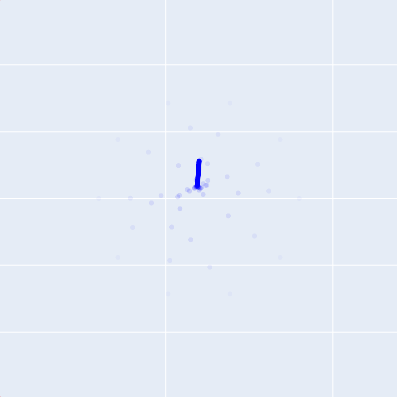
\includegraphics[width=0.32\textwidth]{figures/rendezvous_example_01.png}}  
    \subfigure[]{\label{fig:rendezvous_example_02}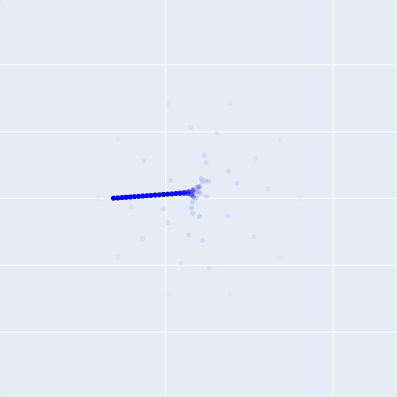
\includegraphics[width=0.32\textwidth]{figures/rendezvous_example_02.png}} 
    \subfigure[]{\label{fig:rendezvous_example_03}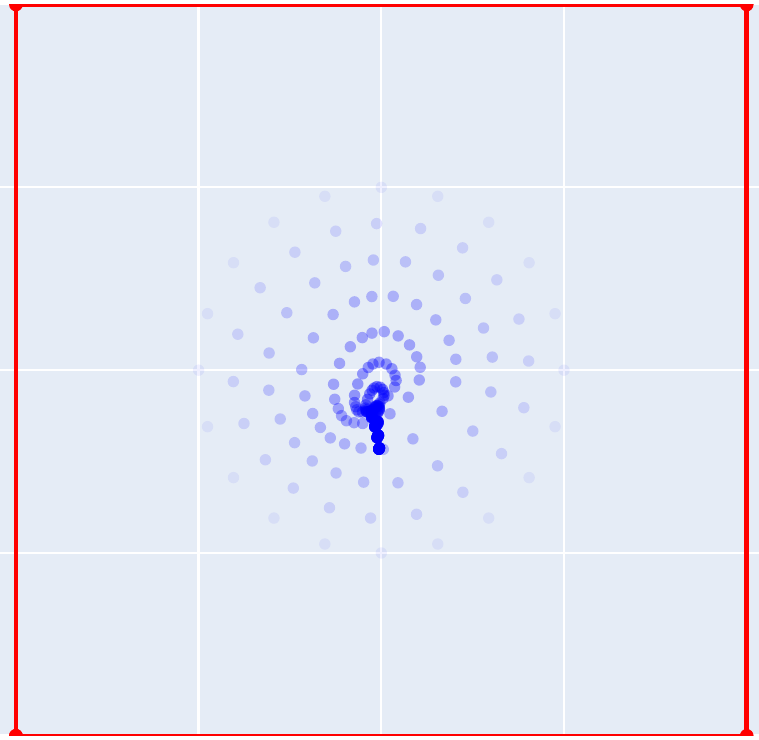
\includegraphics[width=0.32\textwidth]{figures/rendezvous_example_03.png}}   
    \hspace{1cm}                       
    \caption{Three example episodes for Rendezvous. The circular start position used for evaluation can be seen. The agents are able to meed in a couple of steps. Then they move a little as a group.}
    \label{fig:rendezvous_example}
\end{figure}

The goal of the Rendezvous task, is for n agents to converge onto a single point. An example episode can be seen in \Cref{fig:rendezvous_example}.\par

The environment can be configured as a torus (position is wrapped using modulo) or as an rectangular world with borders (position is clipped). Positions are using floating-point precision. It terminates after a given amount of timesteps.
The agents are dots without collisions. They use a direct dynamic model, therefore the two actions they can perform represent movement in the x-Axis and y-Axis respectively.
The reward function $r$ consists of two terms. First we use the mean of the normalized pairwise distances between the agents as a distance penalty $d_p$. Secondly we use an velocity penalty $v_p$, that scales squared to the mean of the velocity $v$:

\begin{equation}
    \begin{aligned}
        v_p &= \textup{mean}(v^2)\\
        d_p &= \textup{mean}(\frac{\textup{pairwise-distances}}{\textup{worldsize}}) \\
        r &= v_p + d_p
    \end{aligned}
    \nonumber
\end{equation}

A culling method is used, so that the agents have a finite sensor range, either kNN or euclidean distance. The observation graph is homogeneous and composed of the following aspects:

\begin{itemize}[noitemsep,nolistsep]
    \item node features:
    \begin{enumerate}[noitemsep,nolistsep]
        \item agent positions, normalized to world size (for debugging, otherwise constant placeholder)
    \end{enumerate} 
    \item edge features:
    \begin{enumerate}[noitemsep,nolistsep]
        \item pairwise agent distances, normalized to world size
    \end{enumerate} 
    \item global features: None
\end{itemize}



\subsection{Dispersion}
\begin{figure}[htp]
    \centering
    \subfigure[$f(x) = \min(x)$]{\label{fig:dispersion_example_01}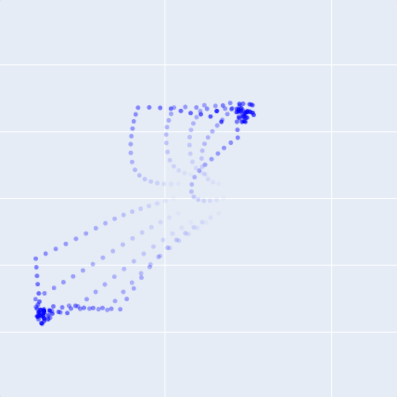
\includegraphics[width=0.32\textwidth]{figures/dispersion_rt_min.png}}  
    \subfigure[$f(x) = x^2$]{\label{fig:dispersion_example_02}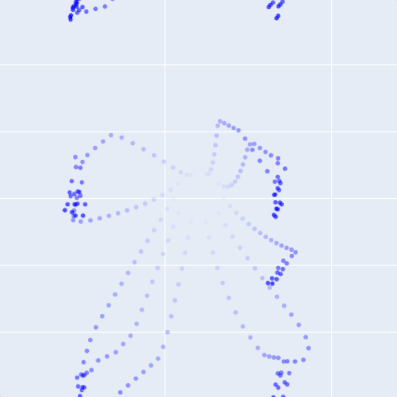
\includegraphics[width=0.32\textwidth]{figures/dispersion_rt_squared.png}} 
    \subfigure[$f(x) = \sqrt(x)$]{\label{fig:dispersion_example_03}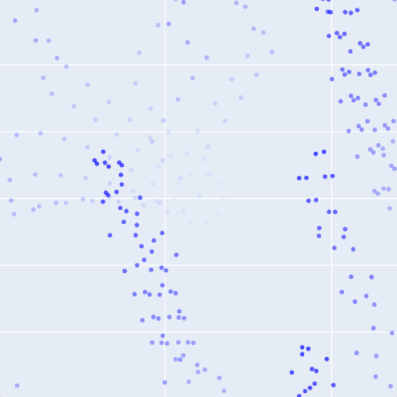
\includegraphics[width=0.32\textwidth]{figures/dispersion_rt_sqrt.png}}   
    \hspace{1cm}                       
    \caption{Three example episodes for Dispersion. The circular start position used for evaluation can be seen. The agents try to disperse and organize into distinct groups. The examples used different reward functions.}
    \label{fig:dispersion_example}
\end{figure}

In a Dispersion task, the agents should try to maximize the distance between each other. An example episode can be seen in \Cref{fig:dispersion_example}.\par

This environment is a variation of Rendezvous and therefore shares most of it's properties. The main difference lies within the reward function $r$. Our implementation allows for different reward calculations using functions $f(x)$ on the reward, before calculating the mean. Supported functions are $x$, $x^2$, $\sqrt{x}$, $\min(x)$, $\max(x)$

\begin{equation}
    \begin{aligned}
        a_p &= \textup{mean}(a^2)\\
        d_p &= \textup{mean}(\frac{f(\textup{pairwise-distances})}{\textup{worldsize}}) \\
        r &= a_p + d_p
    \end{aligned}
    \nonumber
\end{equation}



\subsection{Single Evader Pursuit}
\label{sec:Single Evader Pursuit}


\begin{figure}[htp]
    \centering
    \subfigure[]{\label{fig:single_evader_example_01}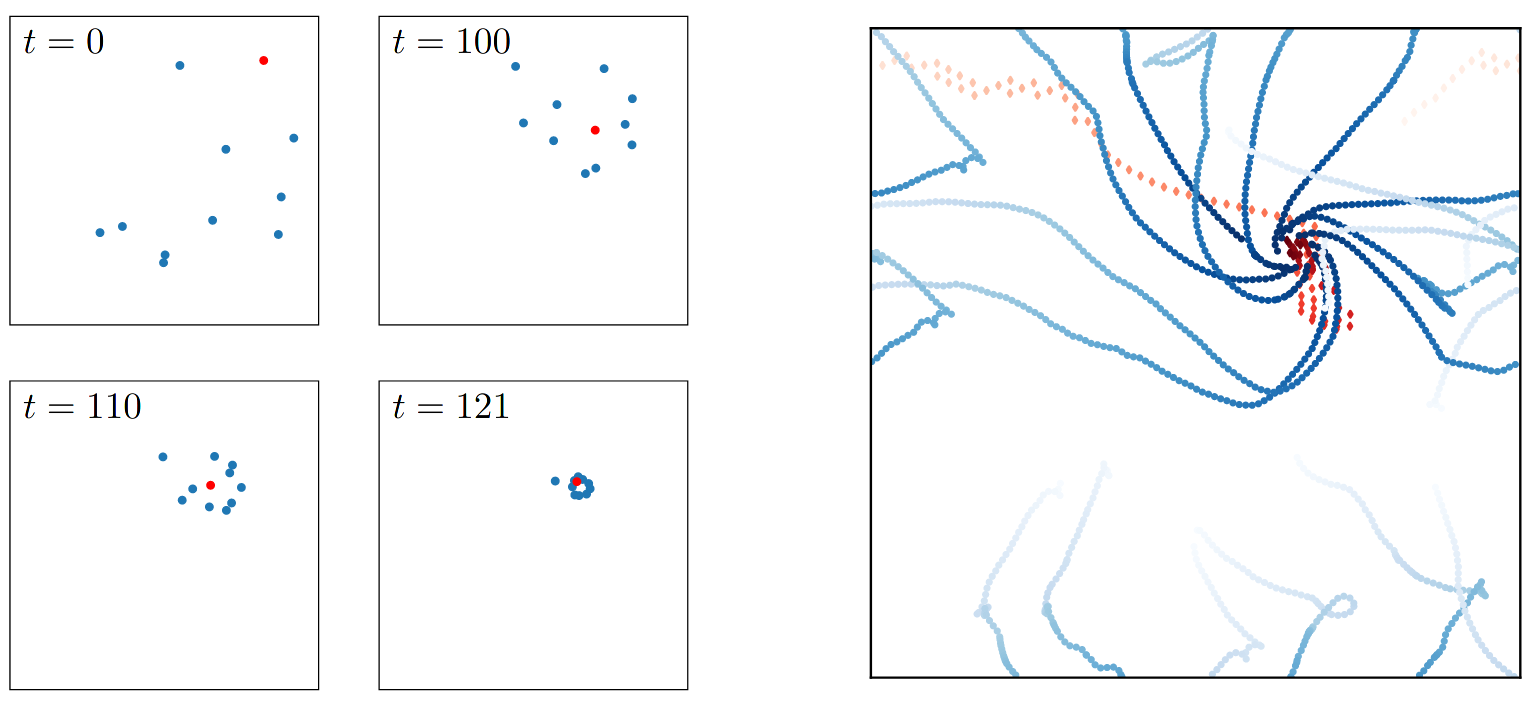
\includegraphics[width=1.0\textwidth]{figures/pursuit_example.png}}  
    \hspace{1cm}                       
    \caption{An example for a successfull Single Evader Pursuit episode, taken from \citet{KIT2019Max}}
    \label{fig:single_evader_example}
\end{figure}

For Single Evader Pursuit the agents have to catch a single evader. Given that the evader has a higher velocity than the agents, they have to cooperate. An example episode can be seen in \Cref{fig:single_evader_example}.\par

The environment can be configured as a torus (position is wrapped using modulo) or as an rectangular world with borders (position is clipped). Positions are using floating-point precision. It terminates after a given amount of timesteps or when the single evader has been caught. A catch is triggered when one agent is less than 1\% of world size away from the evader.
The agents are collisionless dots. Like Rendezvous a direct dynamic model is used. The evader is part of the environment and will not learn. It's dynamic is either a simple linear movement or uses Voronoi-regions which is based on \citet{ZHOU201664}.
The minimum normalized distance of the agents to the evader is used for the distance penalty $d_p$ and the velocity penalty $v_p$ is the same as Rendezvous:

\begin{equation}
    \begin{aligned}
        v_p &= \textup{mean}(v^2)\\
        d_p &= \textup{mean}(\frac{\textup{agent-evader-distances}}{\textup{worldsize}}) \\
        r &= v_p + d_p
    \end{aligned}
    \nonumber
\end{equation}

Single Evader Pursuit also supports the same culling methods as Rendezvous. The observation graph is heterogeneous consists of the following aspects:
\begin{itemize}[noitemsep,nolistsep]
    \item agent node features:
    \begin{enumerate}[noitemsep,nolistsep]
        \item agent positions, normalized to world size  (for debugging, otherwise constant placeholder)
    \end{enumerate} 
    \item evader node features:
    \begin{enumerate}[noitemsep,nolistsep]
        \item evader positions, normalized to world size  (for debugging, otherwise constant placeholder)
    \end{enumerate}
    \item agent-to-agent edge features:
    \begin{enumerate}[noitemsep,nolistsep]
        \item pairwise agent distances, normalized to world size
    \end{enumerate} 
    \item agent-to-evader edge features:
    \begin{enumerate}[noitemsep,nolistsep]
        \item agent to evader distances, normalized to world size
    \end{enumerate} 
    \item global features: None
\end{itemize}



\subsection{Multi Evader Pursuit}

In Multi Evader Pursuit the agents have to catch multiple evaders.\par

This task is largely the same as single evader pursuit. The catch threshhold is changed to less than 2\% of world size.
The reward uses the established velocity penalty $v_p$ and a catch count $c$. It will reward the agents with +1 every time they catch an evader:

\begin{equation} 
    \begin{aligned}
        v_p &= \textup{mean}(v^2)\\
        r &= v_p + c
    \end{aligned}
    \nonumber
\end{equation}